\documentclass{class}

%-----------------------------------------------------------------
\titleind{Laporan Praktikum}

\fullname{Afrizal Dani Saoqi}

\idnum{17/413500/TK/45940}

\papername {Sistem Tertanam dan IoT}

\degree{Teknik Elektro}

\yearsubmit{2020}

\program{Teknik Elektro}

\dept{Teknik Elektro dan Teknologi Informasi}


%-----------------------------------------------------------------



\usepackage[titles]{tocloft}
\renewcommand\cftfigpresnum{Gambar\  }
\renewcommand\cfttabpresnum{Tabel\   }

%Untuk hyperlink dan table of content
\usepackage{hyperref}
\newlength{\mylenf}
\settowidth{\mylenf}{\cftfigpresnum}
\setlength{\cftfignumwidth}{\dimexpr\mylenf+2em}
\setlength{\cfttabnumwidth}{\dimexpr\mylenf+2em}

%Untuk Bold Face pada Keterangan Gambar
\usepackage[labelfont=bf]{caption}

%Untuk caption dan subcaption
\usepackage{caption}
\usepackage{subcaption}
\usepackage{listings}
\usepackage{rotating}
\begin{document}
\cover
    \chapter{Pengenalan}
    \section{Raspberry Pi}
    Raspberry Pi merupakan SBC \emph{(Single Board computer)} yang dikembangkan oleh Raspberry Pi Foundation.
    Pada praktikum ini saya menggunakan Raspberry Pi 3 Model B. Berikut spesifikasi Raspberry Pi 3B dan Pinout GPIO pada Raspberry Pi 3B. \\
    \begin{table}[h!]
      \begin{tabular}{|c|c|c|c|c|c|c|c|}
          \hline
          $SOC$ & Broadcom BCM2837 \\ \hline
          $CPU$ & ARM Cortex A53 64Bit @1.2GHz \\ \hline
          $GPU$ & VideoCore IV @400MHz\\ \hline
          $RAM$ & 1GB LPDDR2 @900MHz\\ \hline
          $Ethernet$ & 10/100Mbps Ethernet\\ \hline
          $Wifi$ & 2.4GHz IEEE 802.11n\\ \hline
          $Bluetooth$ & Bluetooth 4.1 Classic, Bluetooth Low Energy.\\ \hline
          $Storage$ & MicroSD\\ \hline
          $GPIO$ & 40-pin header\\ \hline
          $Max Power$ & 2.5A @5V\\ \hline
          $Ports$ & 4x 2.0 USB Port\\ \hline
          $Video Output$ & 1x HDMI\\ \hline
      \end{tabular}
      \caption{Spesifikasi Raspberry Pi 3B}
  \end{table}
  \begin{figure}[H]
    \centering
        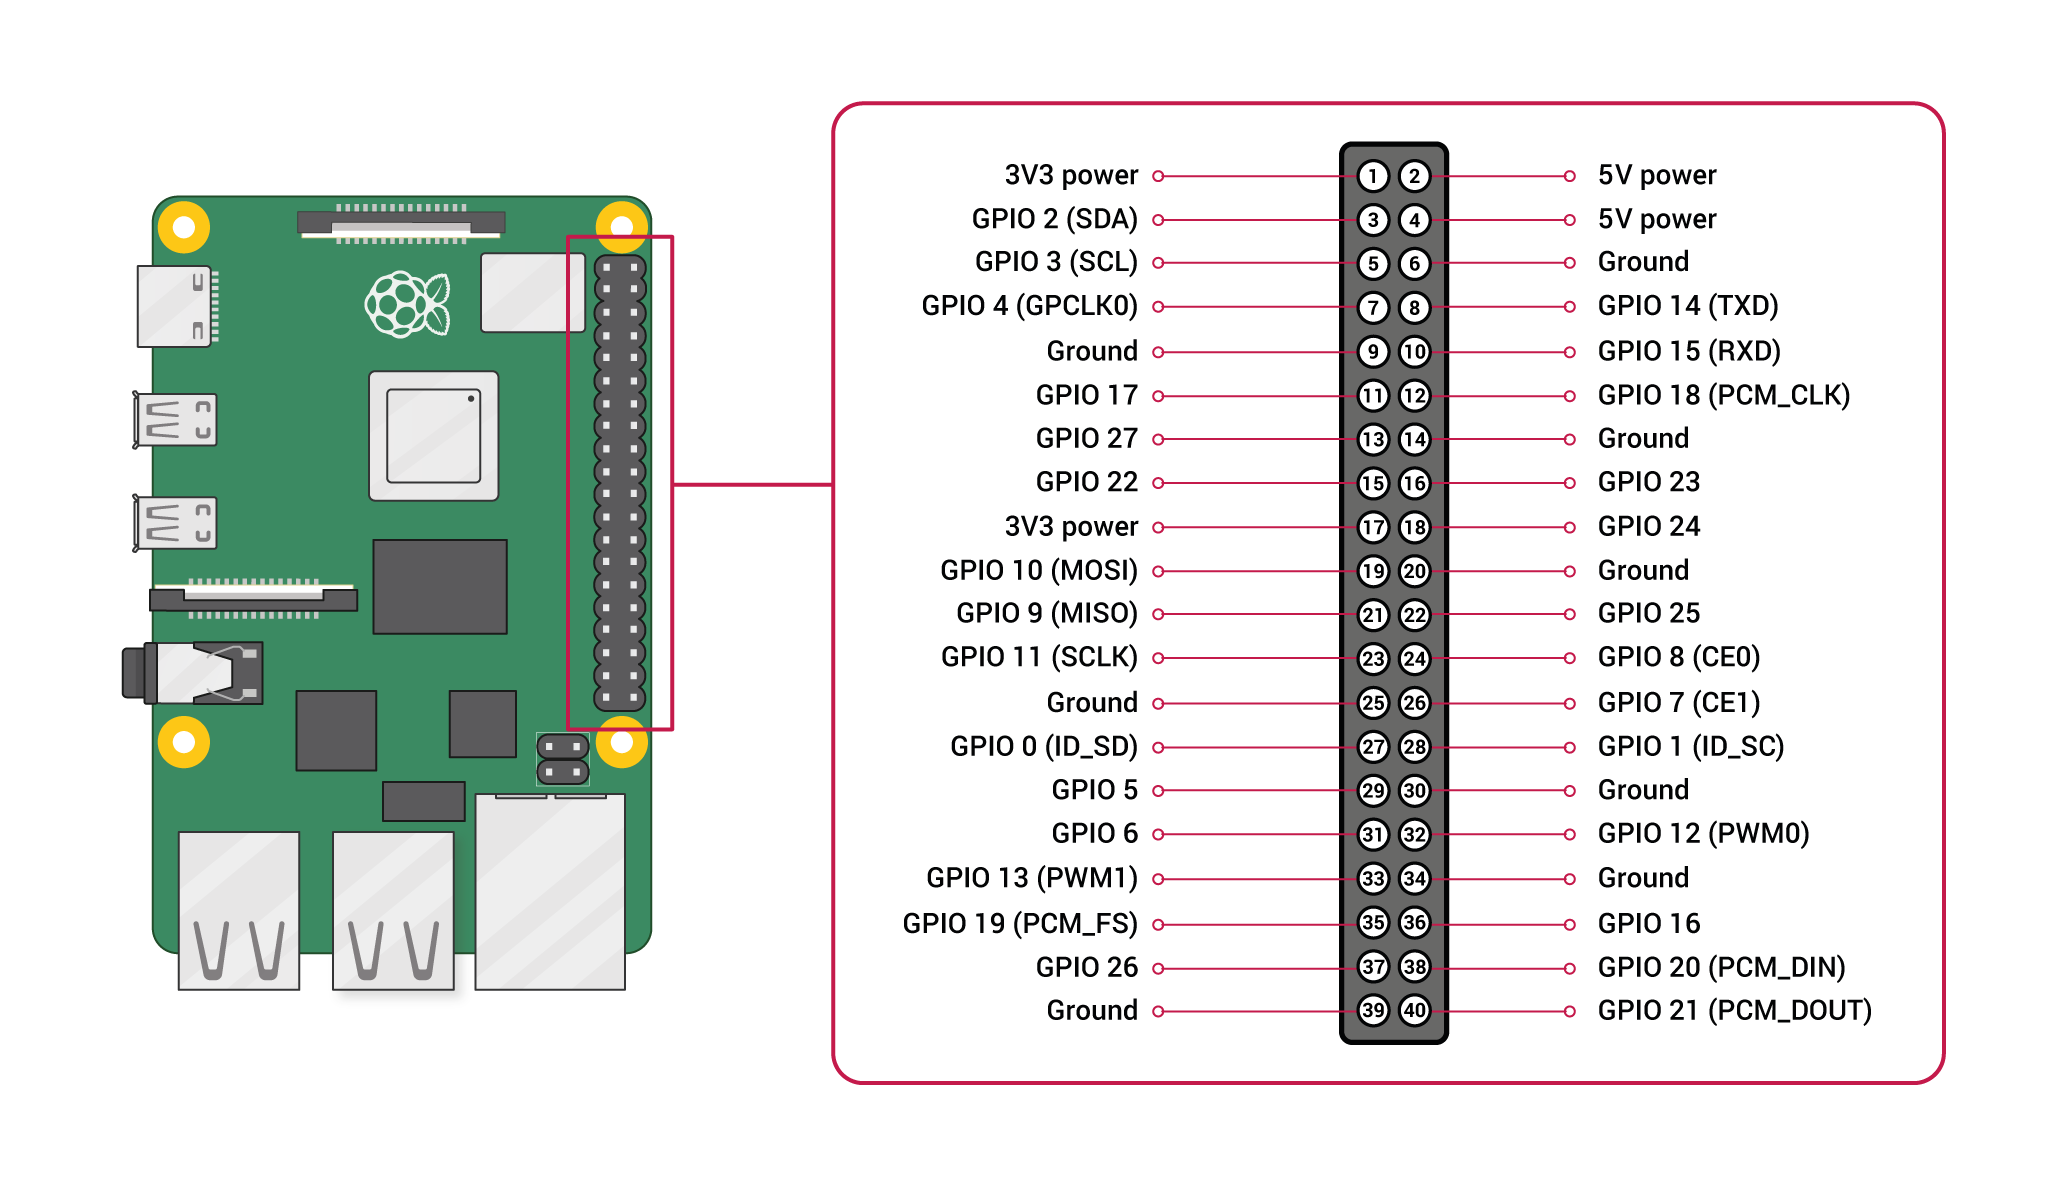
\includegraphics[width=8cm]{gambar/GPIO-Pinout-Diagram-2.png}
        \caption{Pinout Raspberry Pi 3B}
        \label{pinout}
\end{figure}


  \section{NodeMCU}
  NodeMCU adalah mikrokontroler yang dilengkapi dengan modul wifi esp8266. 
  Secara fungsi NodeMCU mirip dengan Arduino, hanya saja NodeMCU sudah dilengkapi dengan wifi.

  \section{Thingsboard}
  Thingsboard merupakan salah satu IoT platform yang open source. 
  Fitur yang terdapat pada thingsboard dapat mempermudah penggguna dalam pengembangan produk, manajemen maupun \emph{scaling} produk. 
  Terdapat 9 menu pada halaman \emph{home}. 
    \begin{enumerate}
      \item HOME
      \item RULE CHAINS
      \item CUSTOMERS
      \item ASSETS
      \item DEVICES \\
      Pada menu ini, pengguna dapat mendaftarkan \emph{device} yang akan digunakan.
      \item ENTITY VIEWS
      \item WIDGETS LIBRARY
      \item DASHBOARDS
      Pada menu ini, pengguna dapat membuat tampilan \emph{dashboard} yang diinginkan
      \item AUDIT LOGS
    \end{enumerate}
  \section{MQTT}
  \section{HTTP}

  \chapter{Pembahasan}
  \section{Praktikum Minggu I}
    \subsection{Percobaan 1}
    Pada percobaan ini, praktikan membuat \emph{device} led pada Thingsboard.
    Setelah membuat \emph{device} maka akan mendapatkan akses token.
    Token tersebut berguna untuk mengakses \emph{device} tersebut.
    \subsection{Percobaan 2}
    Pada percobaan ini, praktikan menginstall \emph{board} NodeMCU dan beberapa \emph{library} yang akan digunakan.
    Terdapat 3 \emph{library} yang digunakan, antara lain:
    \begin{enumerate}
      \item ArduinoJSON
      \item PubSubClient
      \item ESP8266Wifi
    \end{enumerate}
    Source Code
    \begin{enumerate}
      \item \lstinputlisting[firstline=1,lastline=3]{../1/1.ino}
      Kode di atas digunakan untuk menambahkan \emph{library} yang akan digunakan. \\
      \item \lstinputlisting[firstline=5,lastline=12]{../1/1.ino}
      Kode di atas digunakan untuk mendefinisikan sebuah konstanta dan variable. \\
      \item \lstinputlisting[firstline=22,lastline=34]{../1/1.ino}
      Kode di atas digunakan untuk men-\emph{setup} pin, komunikasi serial, komunikasi MQTT, wifi yang akan digunakan. \\
      \item \lstinputlisting[firstline=36,lastline=44]{../1/1.ino}
      Kode di atas digunakan untuk menghubungkan kembali komunikasi mqtt jika terputus.
    \end{enumerate}
    
    \subsection{Percobaan 3}
    Pada percobaan ini, praktikan membuat dashboard yang digunakan untuk mengendalikan led.
    Dashboard tersebut berisi \emph{widget} yang telah diimport

    \subsection{Tugas}
    Terdapat 2 buah led yang dikendalikan melalui dashboard thingsboard. 
    Ketika tombol on pada dashboard thingsboard ditekan maka led pada rangkaian NodeMCU akan menyala, begitu sebaliknya.
    

  \section{Praktikum Minggu II}
  \subsection{Percobaan 1}
    Pada percobaan ini, praktikan membuat \emph{device} DHT11 pada Thingsboard.
    Setelah membuat \emph{device} maka akan mendapatkan akses token.
  \subsection{Percobaan 2}
    Percobaan ini bertujuan untuk mengirim data dari sensor DHT11 ke thingsboard menggunakan mqtt.
    Data yang dikirim adalah nilai dari \emph{Humidity} dan \emph{Temperature}.

  \subsection{Percobaan 3}
  \subsection{Tugas}

    \begin{enumerate}
       
      \item Praktikum Minggu I
      
      Pada praktikum ini, praktikan diminta untuk membuat dashboard yang berfungsi untuk mengontrol pin pada nodemcu.
      $$add \hspace{0.5cm} \$t0, \$t1, \$t2  \hspace{1cm}\$t0 = \$t1 + \$t2$$

      Source Code : 

      \lstinputlisting{code/register.s}
      \begin{figure}[H]
          \centering
              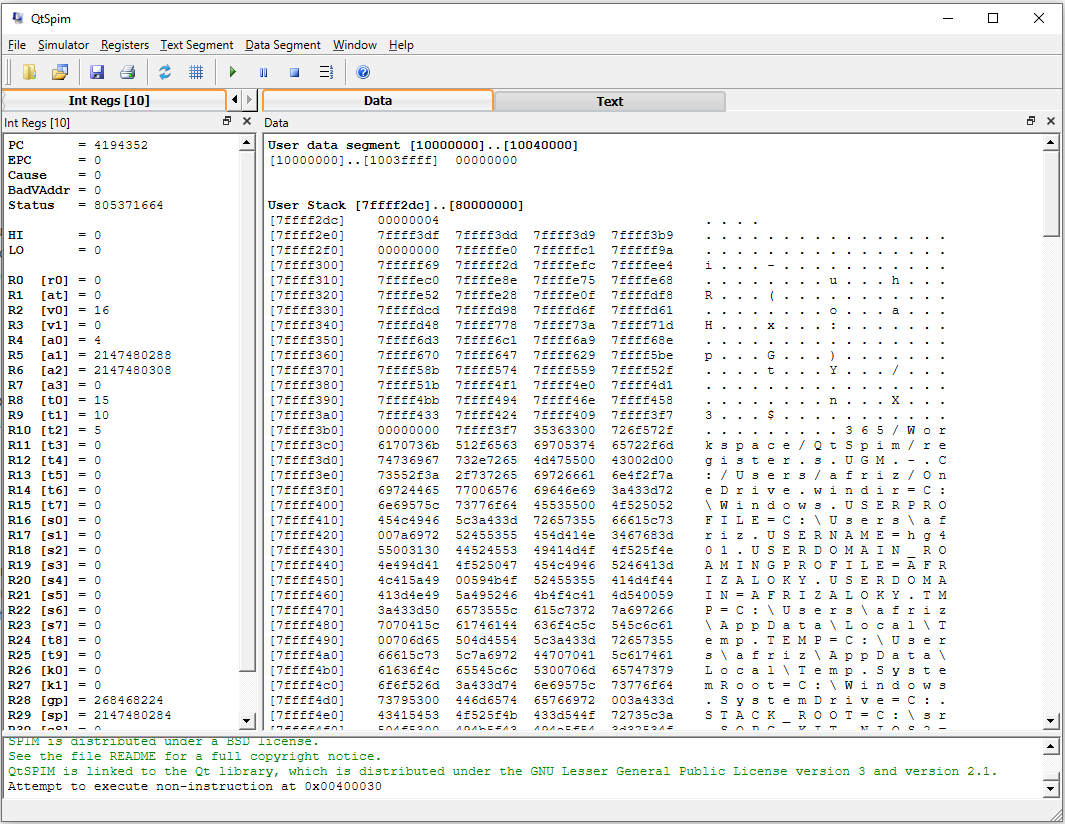
\includegraphics[width=8cm]{gambar/register.png}
              \caption{Simulasi Pengalamatan Register}
              \label{simulasi}
      \end{figure}
      
      Dapat dilihat pada figure 1, nilai t1 adalah 10, nilai t2 adalah 5 dan nilai t0 adalah hasil penjumlahan t1 dan t2.
      \item Pengalamatan Base
      
      Pengalamatan base merupakan pengalamatan yang menunjuk satu pointer sebagai base.
      Dalam pengalamatan ini sebuah register ditunjuk sebagai basis alamat memori
      Contoh dalam penggunaan pengalamatan base : 
      $$lw \hspace{0.5cm} \$s1,4(\$s0)$$
      perintah diatas digunakan untuk mengambil nilai word pada memori s0 dengan offset 4.

      Source Code : 
      \lstinputlisting{code/base.s}
      \begin{figure}[H]
          \centering
              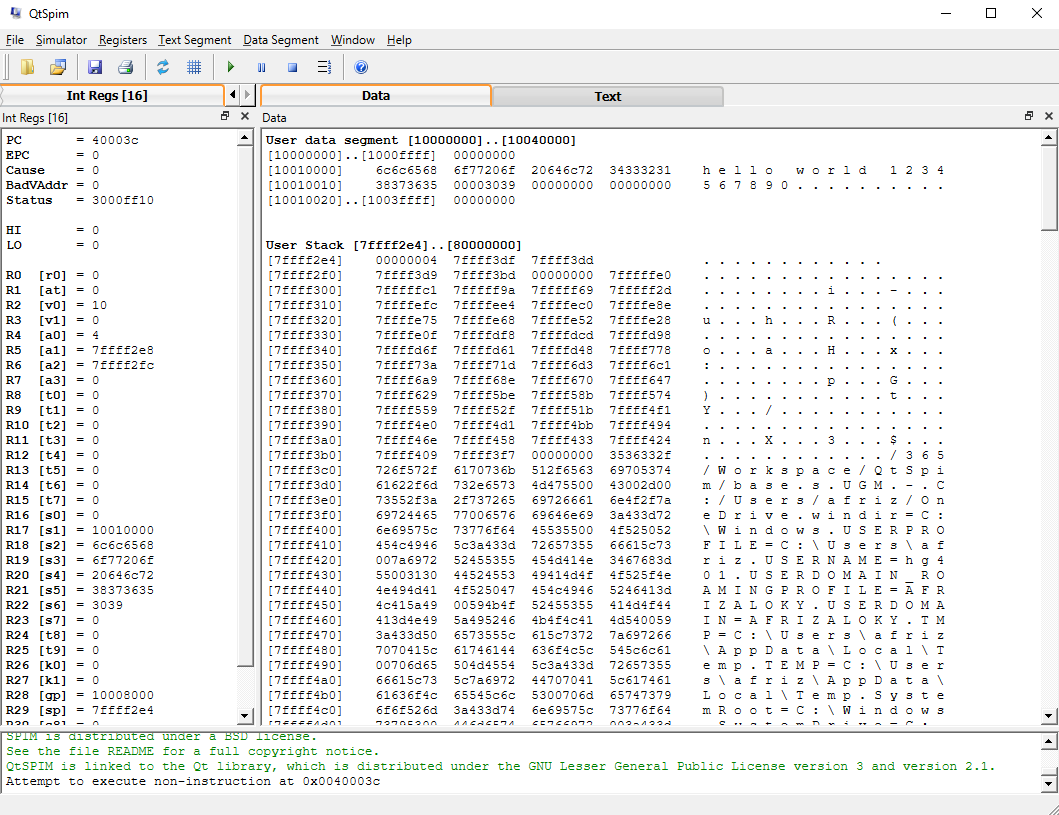
\includegraphics[width=8cm]{gambar/base.png}
              \caption{Simulasi Pengalamatan Base}
              \label{simulasiBase}
      \end{figure}
      
      Pada source code, nilai register s1 adalah sebuah string "hello world"
      Dapat dilihat pada figure 2, register s1 memiliki memory address 0x1001000.
      Register s2 merupakan hasil pointing dari register s1 dengan offset 0. 
      Sehingga register s2 akan memiliki nilai berdasarkan nilai dari memory address 0x1001000-0x1001003.
      Value dari memory address tersebut ditulis dalam format little endian.
      \begin{table}
          \begin{tabular}{|c|c|c|c|c|c|c|c|}
              \hline
              $memory$ & 0x100100 & 0x100101 & 0x100102 & 0x100103 \\ \hline
              $value (hex)$ & 6c & 6c & 65 & 68 \\ \hline
              $value (ascii)$ & l & l & e & h \\ \hline
          \end{tabular}
          \caption{Memory address}
      \end{table}
      
      \item Pengalamatan Immediete
      
      Pengalamatan immediete merupakan pengalamatan yang membutuhkan satu operand saja dan sebuah konstanta (immediete value).
      Pengalamatan ini akan mengeksekusi dirinya sendiri
      Contoh dalam penggunaan pengalamatan immediete :
      $$addi \hspace{0.5cm} \$t0,\$t0,1$$
      Dalam bahasa pemrograman C, kode tersebut dapat ditulis dengan $t0 = t0+1;$

      Source Code : 
      \lstinputlisting{code/immediete.s}
      
      \begin{figure}[H]
          \begin{subfigure}{.5\textwidth}
            \centering
            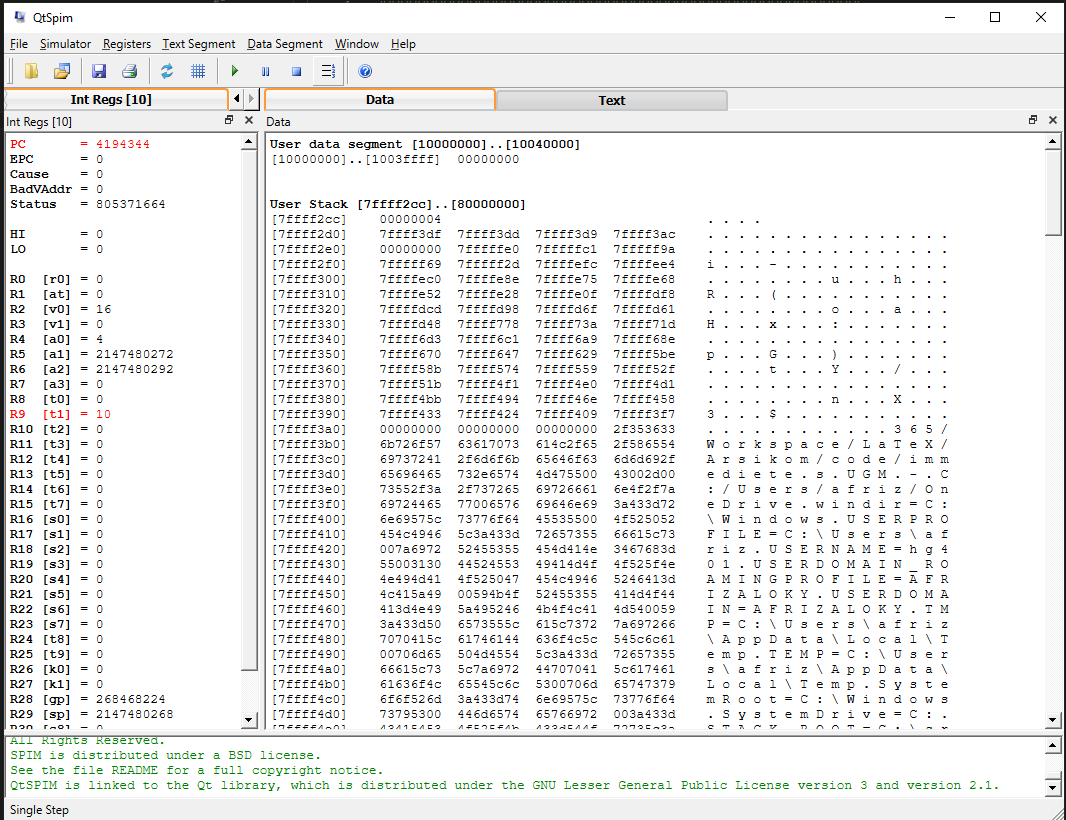
\includegraphics[width=.8\linewidth]{gambar/immediete1.png}
            \caption{step 1}
            \label{immediete1}
          \end{subfigure}
          \begin{subfigure}{.5\textwidth}
            \centering
            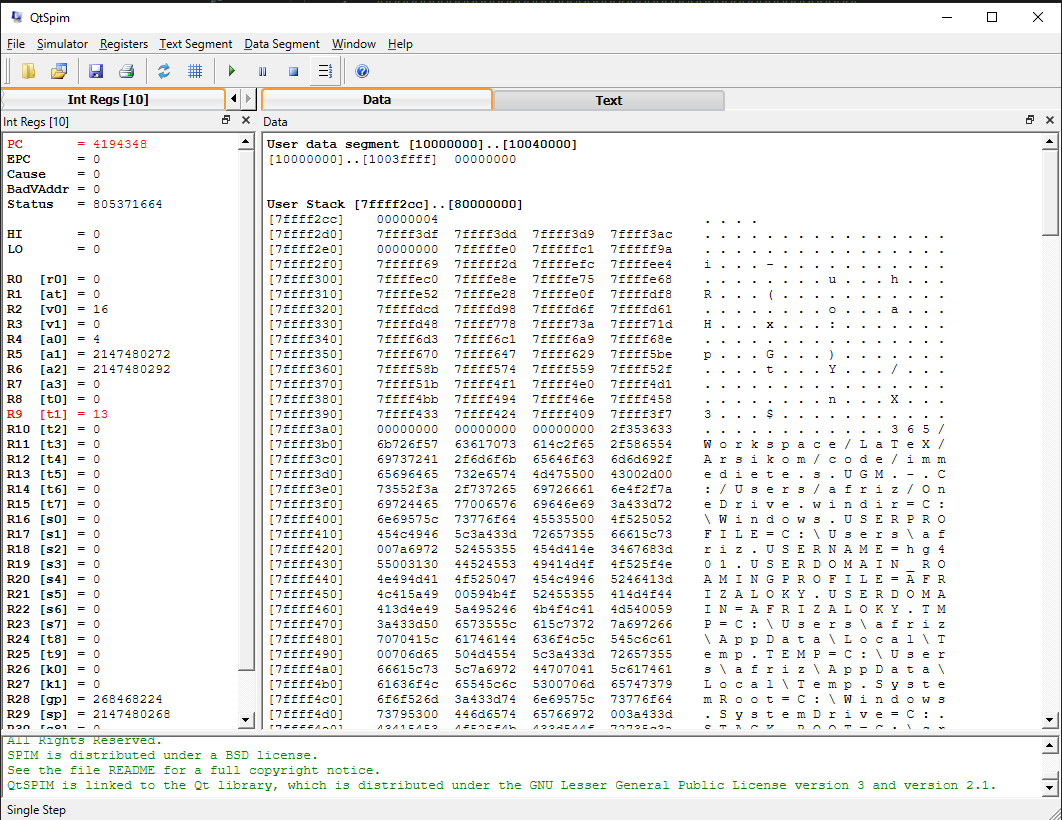
\includegraphics[width=.8\linewidth]{gambar/immediete2.png}
            \caption{step 2}
            \label{immediete2}
          \end{subfigure}
          \caption{Simulasi Pengalamatan Immediete}
          \label{Immediete}
          \end{figure}

      Pada gambar Figure 3.a nilai dari register t1 adalah 10.
      Dengan menggunakan single step pada QtSpim, setelah opcode dieksekusi maka nilai register t1 menjadi 13.
      Hal tersebut dapat dilihat pada gambar Figure 3.b
      \item Pengalamatan PC-relative
      
      % Pengalamatan PC-relative sering disebut juga dengan \emph{Program Counter Addressing}. 
      Data dari pengalamatan ini spesifik pada offset tertentu.
      Pengalamatan ini sering digunakan pada fungsi kondisional.
      Offset value dapat berupa \emph{immediete value} atau sebuah label value.

      Source Code : 

      \lstinputlisting{code/length_pc.s}

      Pada source code tersebut, register t1 merupakan Program Counter.


      \item Pengalamatan Pseudodirect
      
      Pengalamatan pseudodirect biasanya tertanam langsung pada instruksinya. 
      Pseudodirect memiliki instruksi format 6bit untuk opcode dan 26bit untuk target.
      Pseudodirect menggunakan tipe jump instruksi. 

      
      Source Code : 
      \lstinputlisting{code/pseudodirect.s}

      \begin{figure}[H]
          \begin{subfigure}{.5\textwidth}
            \centering
            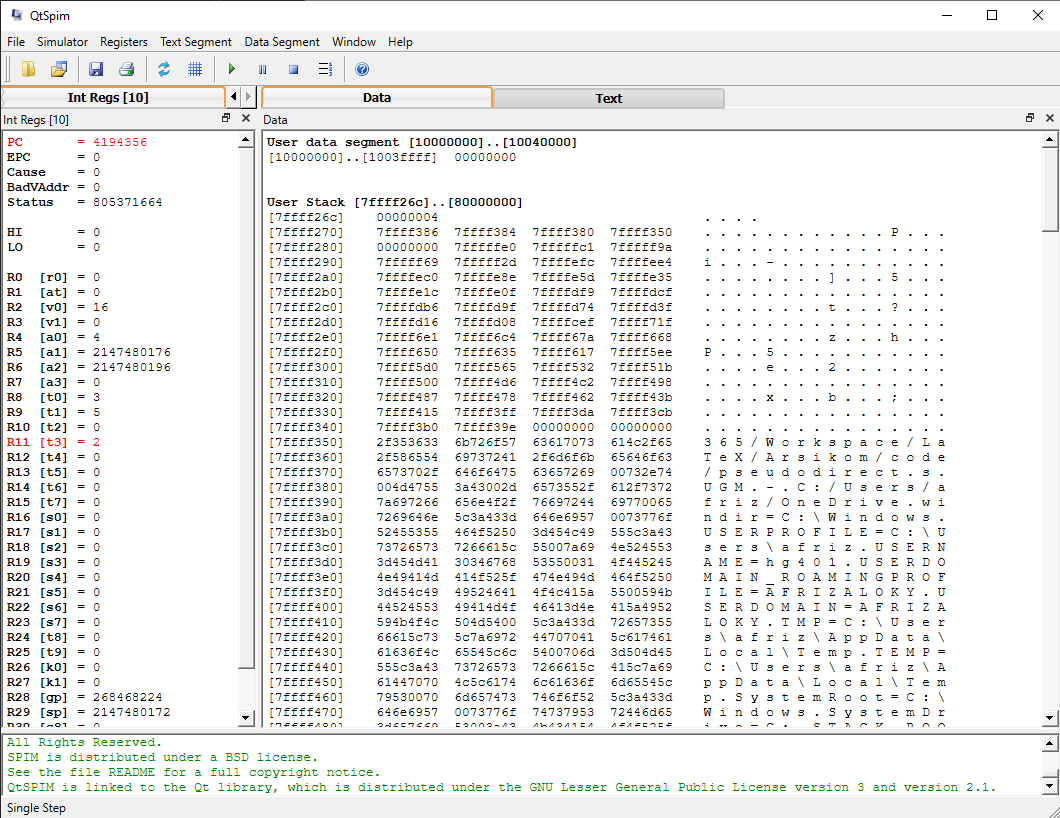
\includegraphics[width=.8\linewidth]{gambar/pseudodirect1.png}
            \caption{step 1}
            \label{pseudodirect1}
          \end{subfigure}
          \begin{subfigure}{.5\textwidth}
            \centering
            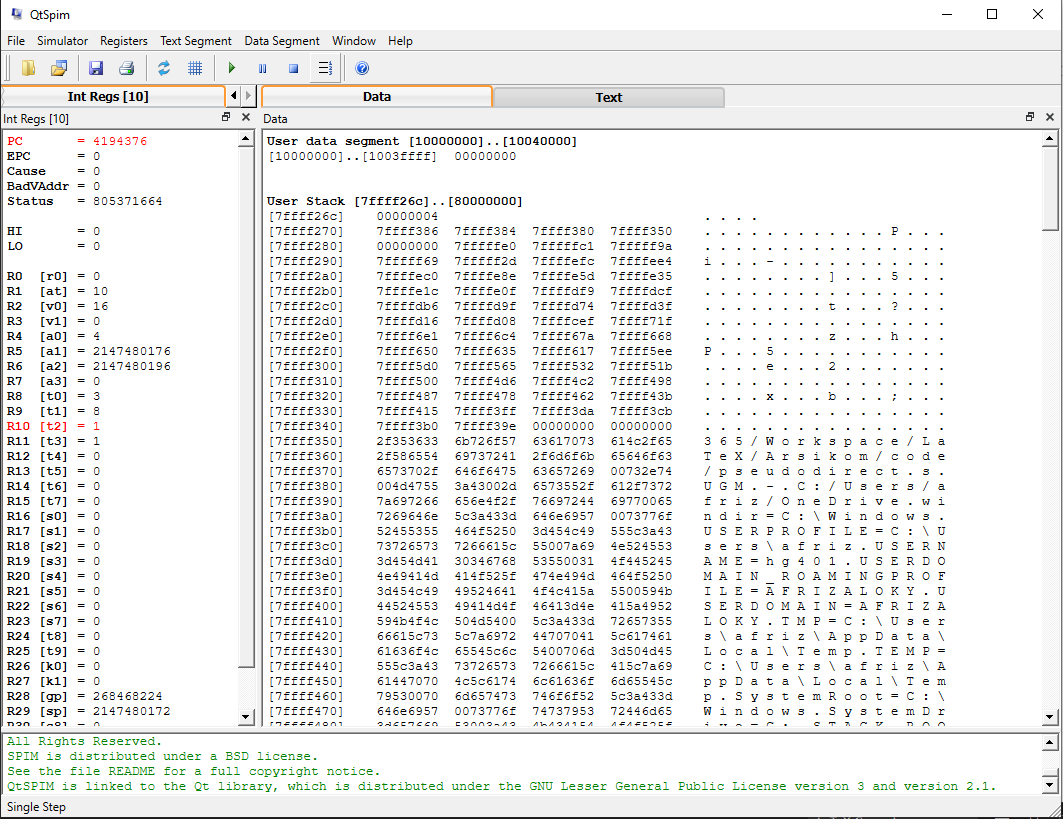
\includegraphics[width=.8\linewidth]{gambar/pseudodirect2.png}
            \caption{step 2}
            \label{pseudodirect2}
          \end{subfigure}
          \begin{subfigure}{0.5\textwidth}
              \centering
              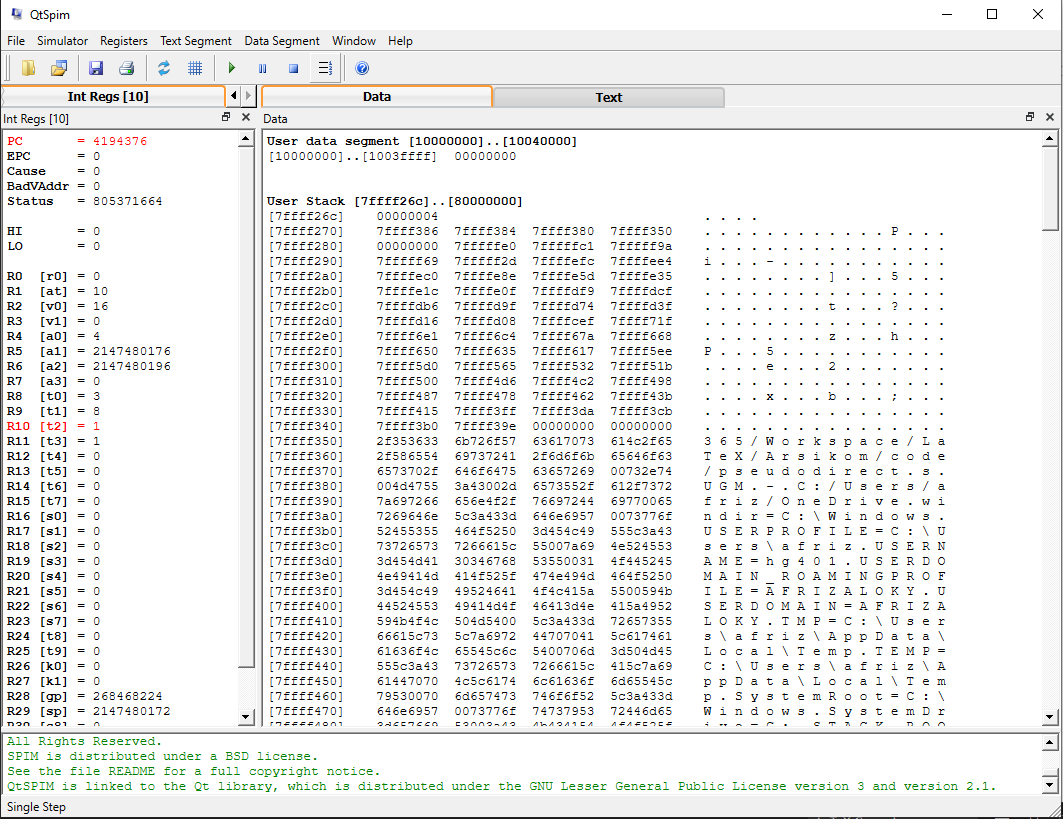
\includegraphics[width=.8\linewidth]{gambar/pseudodirect2.png}
              \caption{step 3}
              \label{pseudodirect2}
            \end{subfigure}
          \caption{Simulasi Pengalamatan pseudodirect}
          \label{Immediete}
          \end{figure}
      
      Pada Gambar 4.a merupakan proses inisiasi nilai register t0,t1,t2 dan t3.
      Pada Gambar 4.b merupakan proses iterasi pertama.
      Pada Gambar 4.c merupakan proses setelah iterasi selesai

      \begin{table}[H]
          \begin{tabular}{|c|c|c|c|c|c|c|c|c|c|c|c|c|}
              \hline
              iterasi ke- & 0 & 1 & 2 & 3 & 4 & 5 & 6 & 7 & 8 & 9 & 10\\ \hline
              $t0$ & 3 & 3 & 3 & 3 & 3 & 3 & 3 & 3 & 3 & 3 &3 \\ \hline
              $t1$ & 5 & 8 & 11 & 14 & 17 & 20 & 23 & 26 & 29 & 32 &35\\ \hline
              $t2$ & 0 & 1 & 2 & 3 & 4 & 5 & 6 & 7 & 8 & 9 & 10 \\ \hline
              $t3$ & 2 & 1 & 0 & -1 & -2 & -3 & -4 & -5 & -6 & -7 & -8 \\ \hline
          \end{tabular}
          \caption{Proses Iterasi}
      \end{table}

\end{enumerate}
\end{document}